\documentclass[11pt,a4paper]{article}
\usepackage[margin=1in]{geometry}
\usepackage{ctex}
\usepackage{setspace}
\usepackage{graphicx}
\usepackage{graphbox}
\usepackage{float}
\usepackage[bookmarksopen=true]{hyperref}
\usepackage{bookmark}
\usepackage{amsmath}
\usepackage{txfonts}
\usepackage{amssymb}
\graphicspath{{graph/}}
%\setmainfont{DengXian}
\renewcommand{\baselinestretch}{1.5}
\begin{document}
\pagestyle{empty}
\begin{titlepage}
    \vspace*{\fill}
    \begin{center}
        \Huge{PJ 中期文档}\\[0.5cm]
        \Large{22302010011 黄宸一}\\[0.4cm]
        \today
    \end{center}
    \vspace*{\fill}
\end{titlepage}
\section*{问题回答}
\subsection*{字母编码}
\par{已知字母a, b, c, d, e, f, g, h出现次数分别为 11, 6, 8, 6, 15, 2, 4, 3,且文件中仅存在这些字母,据此绘制的哈夫曼树如下图:}
\begin{figure}[H]
    \centering
    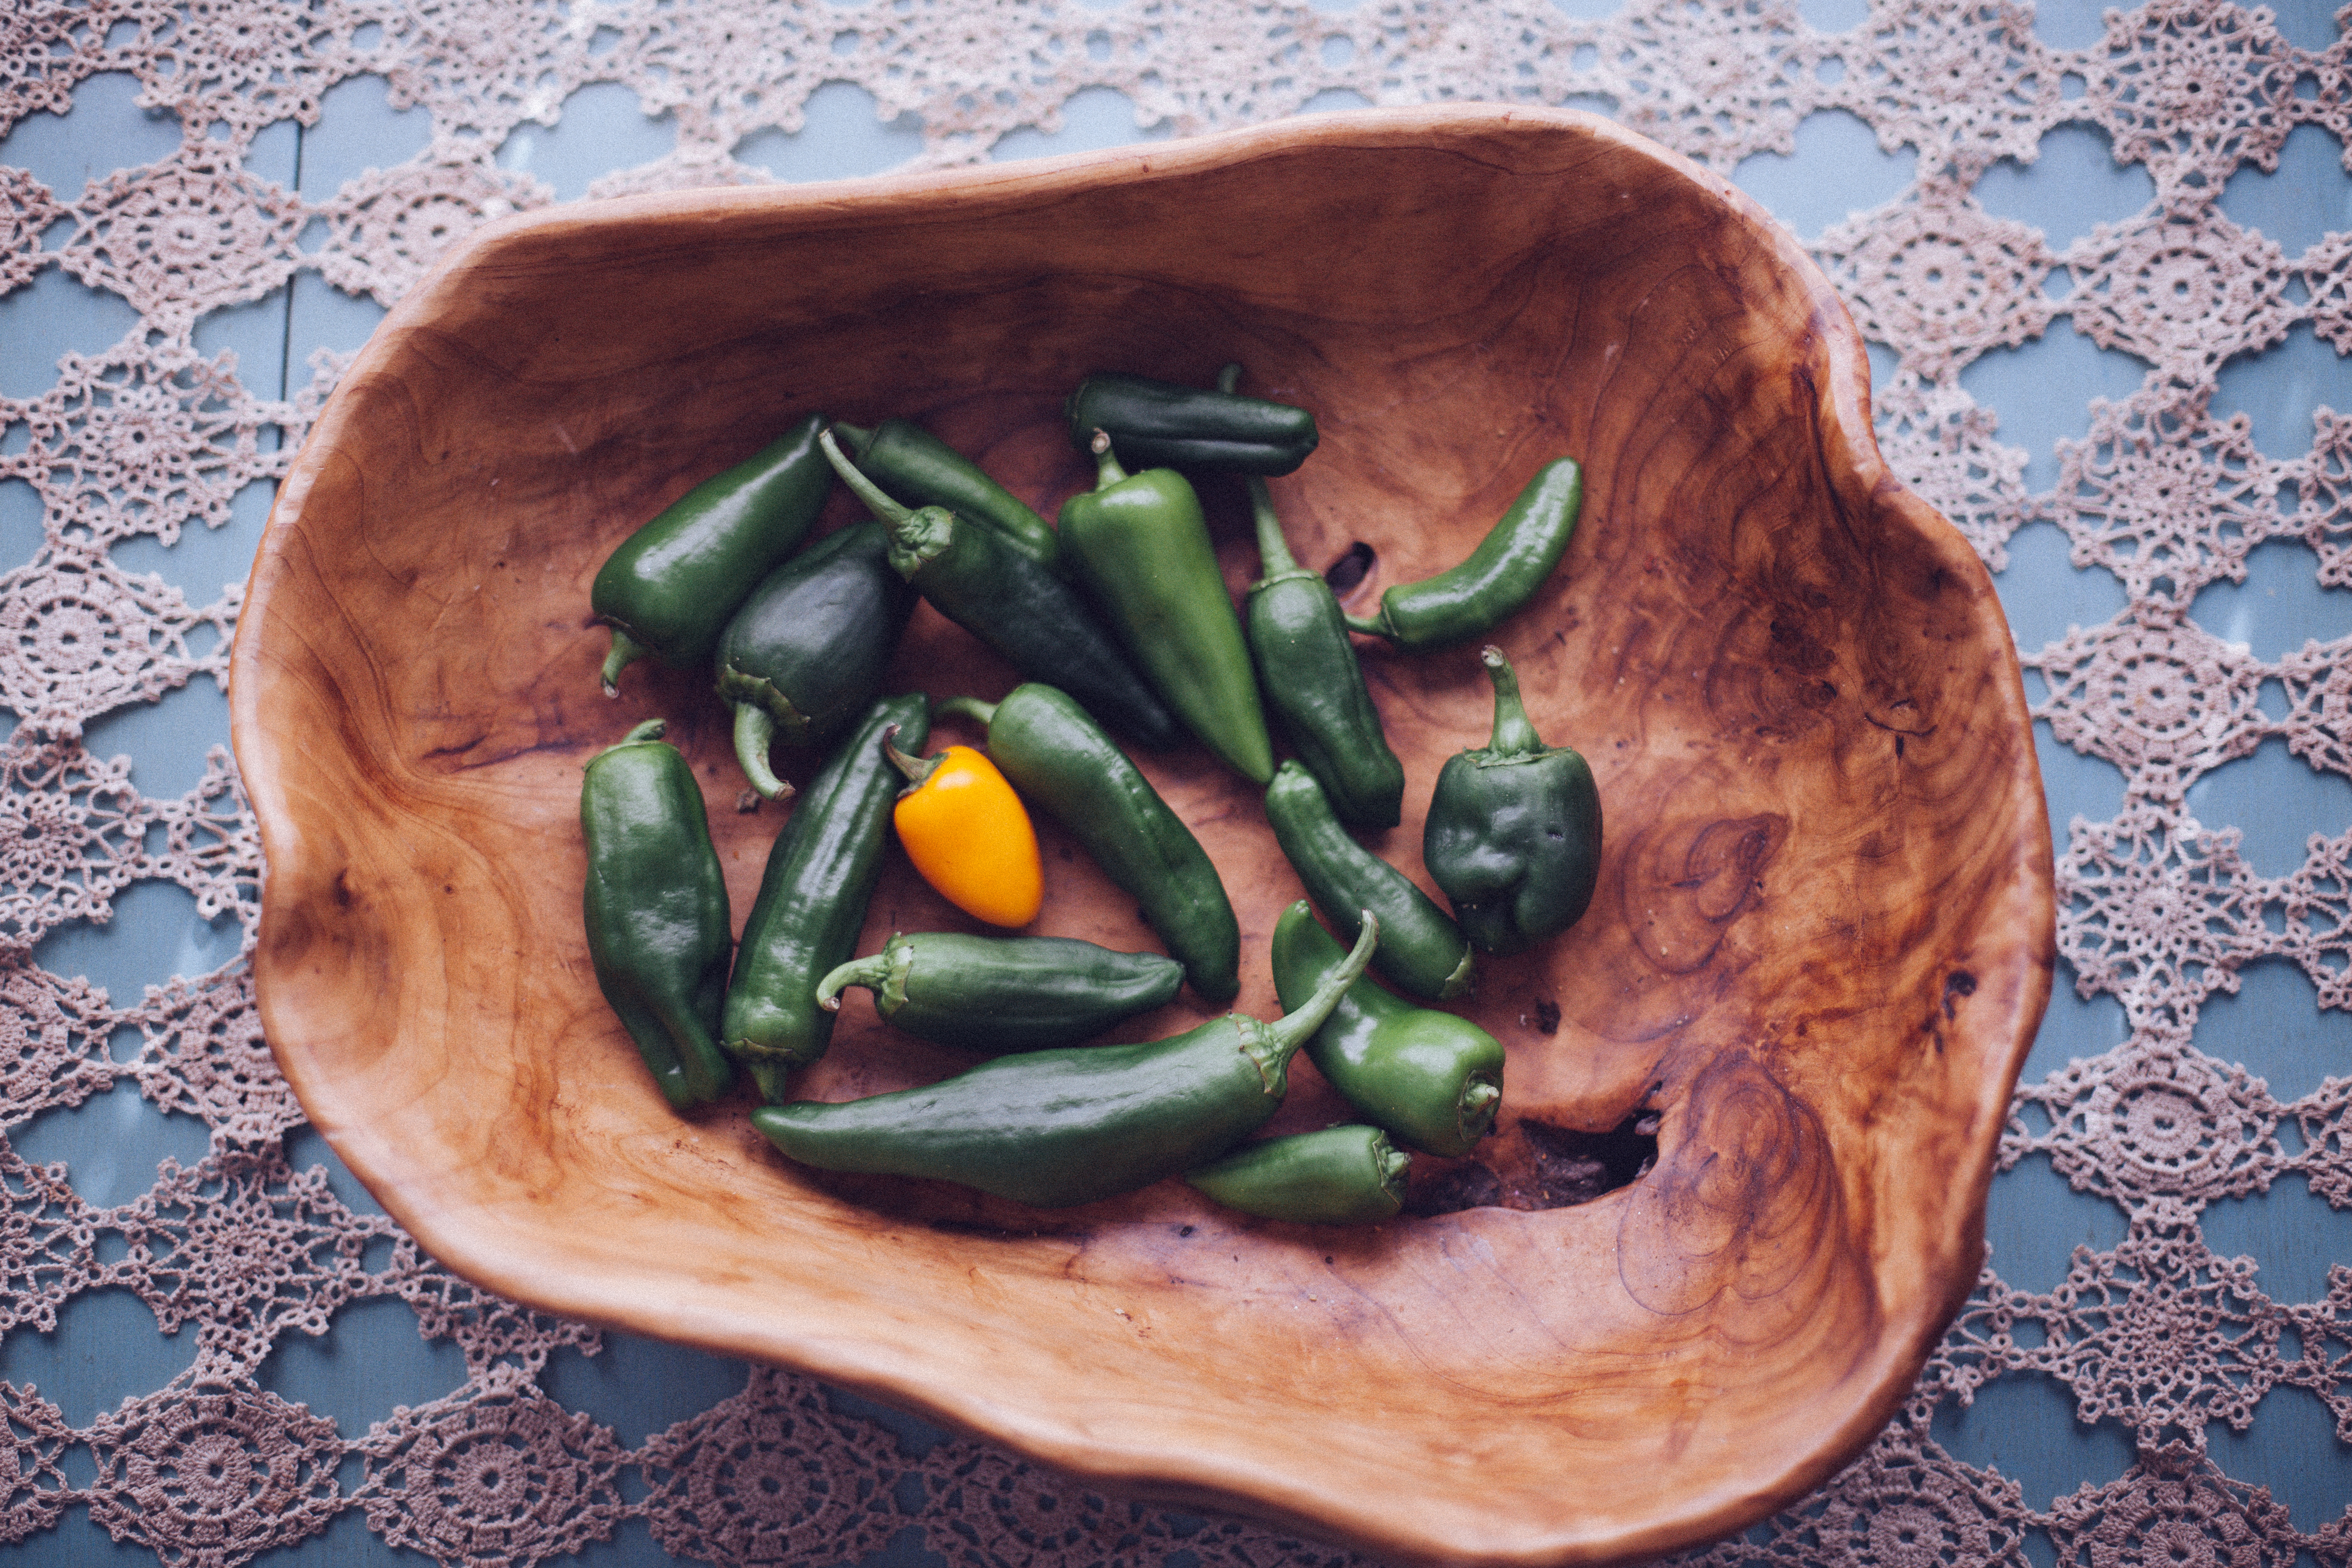
\includegraphics[width=0.7\linewidth]{1.png}
\end{figure}
\par{每个字母对应的哈夫曼编码为:}
\begin{table}[h!]
    \begin{center}
        \begin{tabular}{|l|l|l|} % <-- Alignments: 1st column left, 2nd middle and 3rd right, with vertical lines in between
            a: 00   & b: 010   & c: 110   \\
            d: 011  & e: 10    & f: 11110 \\
            g: 1110 & h: 11111 &          \\
        \end{tabular}
    \end{center}
\end{table}
\subsection*{根据文件字节流构建哈夫曼树}
\par{在我的程序中,使用FileInputStream来按字符(char/8byte)遍历读取文件,当遇到一个第一次出现的字符时,新建以该字符为值的Node型变量。在文件中随机取1000个位置,每取到一个字符,将该字符对应的节点权重加一,经过这一千次更新,每个节点所对应的权重之比就约等于整个文件中各字符出现的频率之比。}
\par{完成节点生成之后,根据哈夫曼树的生成规则,生成新的节点,设置其左右子节点及和权重,最后将整个哈夫曼树的根节点存在HuffmanTree类变量中即可完成哈夫曼树的构建。}
\subsection*{高效选取所需节点}
\par{在遍历完文件第一次生成完节点后,将节点Arraylist按照权重进行排序为升序。之后每一次生成新节点时,先将其放在节点组最后,反复与前一节点权重比较,若比前一节点权重更小,则进行交换,直到达成新的升序节点组,每次只需取节点组中的前两个对象就是出现频率最低的节点。这样只需在最初进行一次全排序,并将每个新节点放到对应位置,而不需每次都再来寻找最小权重节点,较为便捷。}
\subsection*{存储哈夫曼树}
\par{给予HuffmanTree和HuffmanNode以Serializable接口,使用ObjectOutputStream类下的writeObject函数将生成完的哈夫曼树写入文件即可。由于这样存入的哈夫曼树所占大小远小于整个压缩文件的大小,所以直接输出即可,不对其进行其他处理,影响不大。}
\subsection*{保留文件名的文件夹压缩}
\par{本部分还没真正实现,我目前的想法是写一个FileNode类,每个FileNode中包含一个File对象与其文件名,若此对象为文件夹,则在FileNode中存储其子节点,若为文件,则存储其对应的哈夫曼树,最后在文件中先存储最大的FileNode即文件根节点,之后按前序遍历的顺序依次压缩文件存储在目标文件中即可。}
\par{目前对于单个文件的实现方法是把文件名放在huffmanTree对象中一起存储,之后会再作改动。}
\section*{已完成部分说明}
\par{完成了核心需求中的文件压缩解压(在试验中能够压缩解压txt、png、jpg、bmp、mp3、mp4文件,其他格式未试验,但除了txt文件其他格式压缩完的文件都比原来大,之后再研究)、其他需求中的用户交互、检验压缩包来源、文件覆盖问题,下面更细致说明实现思路。}
\subsection*{接收命令}
\par{在main函数中,使用while语句循环接收一行输入,按照空格分隔并存入String数组inputs[]中,直到收到退出命令。使用switch语句对不同的inputs[0]及命令部分调用不同的函数,若命令不为内置的quit、zip、unzip及缩写或者命令所带的参数数量不对则抛出异常,接收异常并输出相应错误提示。}
\subsection*{压缩}
\par{调用checkZip函数。判断变量数是否正确,若不正确则向函数外抛出异常。判断目标文件即inputs[1]是否为huffman文件,若不是则向函数外抛出异常,对所需压缩的文件目前不进行处理与判断。判断所压文件是否存在,若不存在,同样抛出异常。}
\par{检测目标文件即被压缩文件inputs[1]是否已经存在,若不存在则直接调用zip函数,若已存在,则询问是否需要覆盖,选择覆盖后将原来已存在的文件删除,调用zip函数进行压缩。}
\par{正式进入压缩过程。遍历文件获取节点组、生成哈夫曼树及文件名存储的部分上面已经说过,不再赘述。在向文件写入哈夫曼树对象后调用huffmanTree.generateAllCode()函数,递归生成树中每一节点所对应的01编码,此处的目的是之后每次寻找对应编码时只需在最初的节点组找到字符对应节点调取其编码即可,而不用每次都在整个哈夫曼树中寻找,更为高效。再次遍历整个文件,对每一个字符,调取其对应编码连接在一起,每8位转化为一个字节即8bit写入目标文件中。最后需要注意的是在这一转化过程中最后可能会剩余小于8位的编码串,若也直接转换成字节写入,在解压时就不知道哪一位是最后一位,因此我选择的方法是在最后一位后补上1-8位与最后一位相反的数字,如若剩余00101,则补为00101000,若剩余11010100(即刚好填满),则在后面再补上8个1。}
\par{另外,在上面两次遍历文件的过程中我都插入了一个变量now,代表当前读到的位置,通过now与文件总长的的计算在终端显示出当前压缩过程百分比。我还在zip函数的开头与结尾处记录了当前时间,相减得到压缩时间作为zip函数的输出,最后在压缩完毕后显示在终端中,同时将压缩后文件长度与压缩前文件长度相除得到压缩率也显示在终端中。}
\subsection*{解压}
\par{调用checkUnzip函数,同样判断变量数是否正确,若不正确则抛出异常。判断所需解压文件是否为huffman文件,若不是则抛出异常说明不可解压。判断所解压文件是否存在,若不存在,同样抛出异常。}
\par{首先读取文件开头的huffmanTree对象,从其中调取压缩前文件的文件名,判断该文件是否已存在,询问是否需覆盖,生成目标文件,调用unzip函数,不过多叙述。}
\par{正式进入解压过程。按字符读取被解压文件并转化为二进制01序列,按照该序列移动节点nodeNow,0代表移动到左子节点,1代表移动到右子节点,若移动到了无子节点的节点,则取该节点的字符值写入目标文件中并将nodeNow取回哈夫曼树的根节点,如此循环直到剩下的序列全为0或1,说明该文件已到末尾,后面的这些序列是需要被舍弃的,完成解压。}
\par{同样,我设置了变量now用来计算显示当前解压进度,并在unzip函数的开头与结尾处记录了当前时间,相减得到压缩时间作为unzip函数的输出,最后在解压完毕后显示在终端中。}
\subsection*{关于空文件}
\par{目前的实现方式为在zip函数中首先检测是否为空文件即file.length()是否为0,若是则直接向目标文件中存入一个仅存有文件名而根节点为null的哈夫曼树,结束压缩。解压时在创建文件后只需判断若根节点为空则说明为空文件,直接结束解压即可。不过这里涉及到在哈夫曼树中存储的文件名,后续进行关于FileNode改动后这里会有一定改变,在最终文档中再说明。}
\subsection*{关于时间}
\par{目前压缩时间我认为较长,txt文件压缩约3mb/s,还有优化的空间,或许可以一次多读进缓冲一些字符,但还未进行尝试。}
\end{document}